%
% ---------------------------------------------------
%
% Proyecto Final de Carrera: EMIR
% Autor: Pedro Hernández Martín <alu3679@etsii.ull.es>
% Capítulo: Estado del arte
% Fichero: Cap_aplicacion.tex
%
% ----------------------------------------------------
%

\chapter{La Aplicación \CSUO{}} \label{chap:aplication}
En este capítulo se explica en detalle la aplicación \CSUO{}, cómo
instalarla, cómo funciona, qué opciones tiene disponibles, etc. 
\CSUO{} ha sido desarrollada en C++ sobre una plataforma Linux, más
concretamente una distribución Ubuntu. 
En este Capítulo asumiremos que el usuario final dispone de un PC con esta distribución instalada y operativa.

La aplicación se entrega con la siguiente estructura de directorios:

\begin{itemize}
\item \texttt{bin}: Aplicación \CSUO{}.
\item \texttt{documentacion}: Documentación de código generada con Doxygen.
\item \texttt{ejemplos}: Algunos ejemplos de entrada.
  \begin{itemize}
  \item \texttt{conversor}: Aplicación para convertir archivos.
  \item \texttt{xml}: Ficheros XML correspondientes a los ejemplos.
  \end{itemize}
\item \texttt{map\_editor}: Aplicación para generar ejemplos sintéticos.
\item \texttt{memoriaEmir}: Código LaTEX de este documento.
\item \texttt{Resultados}: Ficheros de resultados de la aplicación.
\end{itemize}

Para la implementación de la aplicación se barajaron dos lenguajes de
programación, JAVA y C++, siendo elegido el segundo debido a la importancia
de una respuesta rápida a la hora de obtener soluciones por parte de la aplicación.
Se ha preferido utilizar un lenguaje compilado frente a uno interpretado en un intento
de satisfacer este requisito.
%%%%%%%%%%%%%%%%%%%%%%%%%%%%%%%
\section{Repositorio de código}
El código de la aplicación, así como el manual de la misma, se encuentra disponible en un
repositorio remoto alojado en Bitbucket \cite{Web:BIT} del que es posible descargarla.
Bitbucket es un servicio
de alojamiento basado en web, para proyectos que utilizan el sistema de
control de versiones Mercurial y/o Git. 
En el caso de este PFC hemos optado por utilizar Mercurial \cite{Web:MERCURIAL}.

%%%%%%%%%%%%%%%%%%%%%%%%%%%%%%%
\section{Instalación}
\subsection{Dependencias}
Antes de instalar la aplicación ha de asegurarse que se satisfacen todas las dependencias
de la misma, que se enumeran a continuación:
%%%%%%%%%%%%%%%%%%%%%%%%%%%%%%%
\subsubsection{make}
La herramienta make es necesaria para la automatización del compilado. Puede
instalarse desde la consola mediante:
\begin{lstlisting}[numbers=none]
sudo apt-get install make
\end{lstlisting}

%%%%%%%%%%%%%%%%%%%%%%%%%%%%%%%
\subsubsection{Compilador de C++}
El compilador \texttt{g++} es imprescindible para poder compilar el código.
Normalmente viene instalado por defecto en cualquier distribución Linux, pero si no fuera el caso, se puede
instalar usando:
\begin{lstlisting}[numbers=none]
sudo apt-get install g++
\end{lstlisting}
%%%%%%%%%%%%%%%%%%%%%%%%%%%%%%%
\subsubsection{libxml++}
Ésta librería es el parser XML que se ha usado con aplicación, tal y como se ha descrito en 
la Sección \ref{sec:LIBXML}. 
Para instalar \texttt{libxml++} se precisan los siguientes comandos:
\begin{lstlisting}[numbers=none]
sudo apt-get install libxml++2.6-dev libxml++2.6-doc
sudo apt-get install libgtkmm-2.4-dev
\end{lstlisting}
%%%%%%%%%%%%%%%%%%%%%%%%%%%%%%%
\subsubsection{Doxygen}
Doxygen \cite{Web:DOX} es un acrónimo de dox(document) gen(generator), generador de
documentación para código fuente.
Se trata de un generador de documentación para diversos lenguajes, entre ellos C++, C, o Java.
Dado que es fácilmente adaptable, funciona en la mayoría de
sistemas Unix así como en Windows y Mac OS X. 
La mayor parte del código de Doxygen ha sido escrito por Dimitri van Heesch.
Varios proyectos como KDE usan Doxygen para generar la documentación de su API.
KDevelop incluye soporte para Doxygen.

Para descargar Doxygen e intalarlo han de seguirse estos pasos:
\begin{itemize}
  \item Descargar y descomprimir el código fuente:
\end{itemize}
\begin{lstlisting}[numbers=none]
wget http://ftp.stack.nl/pub/users/dimitri/doxygen-1.8.4.src.tar.gz
tar -xzvf doxygen-1.8.4.src.tar.gz
\end{lstlisting}
\begin{itemize}
  \item Situarse en el directorio generado e intentar pre-instalar
    \begin{lstlisting}[numbers=none]
cd doxygen-1.8.4/
./configure
    \end{lstlisting}
  \item Si falla alguna de las comprobaciones, instalar dependencias.
    \begin{itemize}
      \item para graphviz:
        \begin{lstlisting}[numbers=none]
sudo apt-get install graphviz
        \end{lstlisting}
      \item para flex:
        \begin{lstlisting}[numbers=none]
sudo apt-get install flex
        \end{lstlisting}
      \item para bison:
        \begin{lstlisting}[numbers=none]
sudo apt-get install bison
        \end{lstlisting}
    \end{itemize}
  \item Una vez ejecutado el \texttt{./configure}
    \begin{lstlisting}[numbers=none]
make
sudo make install
    \end{lstlisting}
\end{itemize}

%%%%%%%%%%%%%%%%%%%%%%%%%%%%%%%
\subsubsection{LaTeX}
LaTeX \cite{Web:LATEX} es un sistema de composición de textos orientado
especialmente a la creación de libros, documentos científicos y técnicos.
LaTeX está formado por un gran conjunto de macros de TeX, escrito por Leslie
Lamport en 1984, con la intención de facilitar el uso del lenguaje de
composición tipográfica, TEX, creado por Donald Knuth. 
Es bien conocido en entornos académicos y científicos en los que 
la calidad tipográfica de los documentos generados es muy apreciada.
LaTeX es software libre bajo licencia LPPL.

Esta herramienta únicamente es necesaria si se necesita generar este documento, y
es posible instalarla con:
\begin{lstlisting}[numbers=none]
sudo apt-get install texlive-extra-utils
sudo apt-get install texlive-latex-extra
sudo apt-get install texlive-latex-recommended
sudo apt-get install texlive-full
sudo apt-get install texlive-science
\end{lstlisting}

%%%%%%%%%%%%%%%%%%%%%%%%%%%%%%%
\subsubsection{Allegro}
La librería Allegro, descrita en la Sección \ref{sec:Allegro}, se utiliza en el
\CSUO{} para la representación gráfica de los apuntados.

Para instalar Allegro se debe utilizar el siguiente paquete:
\begin{lstlisting}[numbers=none]
sudo apt-get install liballegro4.2-dev
\end{lstlisting}

Para utilizar Allegro en el código, basta con incluir el fichero de cabecera
\texttt{allegro.h} en el código tal como se muestra en la línea 1 del Listado \ref{codigo:allegro0}.
Este listado muestra cómo utilizar \texttt{Allegro} para inicializar y crear
una ventana.
\begin{lstlisting}[language=C++,basicstyle=\ttfamily\footnotesize,
                   caption={Ejemplo básico de uso de la librería Allegro},
                   label={codigo:allegro0}]
#include <allegro.h>
// Para poder cerrar la ventana pulsando el boton de cerrar
volatile int close_button_pressed = FALSE;
void close_button_handler(void) {
  close_button_pressed = TRUE;
}

int main (int argc, char **argv) {
  allegro_init(); // Inicializamos allegro
  install_keyboard();
  set_color_depth(16);
  set_window_title("Nombre de la ventana");
  // Definimos los tamanios de la ventana (800x800) pixeles de resolucion
  int w = 800, h = 800;
  //Generamos la ventana
  if(set_gfx_mode(GFX_AUTODETECT_WINDOWED,w,h,0,0) != 0) { //modo grafico
    set_gfx_mode(GFX_TEXT,0,0,0,0);
    allegro_message("imposible iniciar el modo video\\n\%s\\n",allegro_error);
    return 1;
  }
  clear_bitmap(screen);  // Limpiamos la pantalla
  while (!key[KEY_ESC]&&!close_button_pressed) {}
}
\end{lstlisting}

Si lo que se desea es dibujar puntos o líneas, se debe crear un nuevo BITMAP
sobre el que dibujar, modificarlo, y luego enviarlo a la pantalla. 
El Listado \ref{codigo:allegro1} muestra un ejemplo de cómo hacerlo.

\begin{lstlisting}[language=C++, basicstyle=\ttfamily\footnotesize,
                   caption={Ejemplo de dibujo con Allegro},
                   label={codigo:allegro1}]
BITMAP* bmp = create_bitmap(ancho, alto);
// Creamos una linea roja de (x1,y1) a (x2,y2)
line(bmp, x1, y1, x2,y2,makecol(255,0,0));
// Creamos un punto azul de 4 pixeles de radio en (x,y)
circlefill(bmp, x, y, 4, makecol(0,0,255));
// Enviamos lo pintado en bmp a la pantalla
stretch_blit(bmp, screen, 0,0,bmp->w, bmp->h, 0,0, SCREEN_W, SCREEN_H);
\end{lstlisting}

Estas dos combinaciones son capaces de dibujar tanto los elementos que forman el
problema como los apuntados que lo solucionan.
%%%%%%%%%%%%%%%%%%%%%%%%%%%%%%%
\subsection{Instalación}
Una vez comprobadas las dependencias, no hay más que descargar (bien descargando
el fichero \texttt{.tar.gz}, o bien clonando el repositorio) y descomprimir el fichero del
proyecto. 
Para compilar la aplicación y utilizarla basta con ejecutar:

\begin{lstlisting}[numbers=none]
cd bin/
make
\end{lstlisting} 

Esto creará el archivo ejecutable \texttt{csuoptimizer}. 
Para comprobar que funciona correctamente se puede probar con alguno de los ejemplos incluidos en
el directorio \texttt{ejemplos/xml/}.

\begin{lstlisting}[numbers=none]
./csuoptimizer ../ejemplos/xml/exacto.xml
\end{lstlisting} 

La salida debería ser igual a la mostrada en la Figura \ref{fig:exacto-out}.

%%%%%%%%%%%%%%%%%%%%%%%%%%%%%%%
\section{\CSUO{}}
\CSUO{} utiliza cinco clases, una de configuración y cuatro de estructuras. 
La clase de configuración tiene como finalidad establecer opciones
entre todas las instancias del resto de las clases, según las necesidades del
usuario. En esta sección se explicará cada una de estas estructuras, detallando
el significado de los atributos de cada clase y el funcionamiento de los métodos más
relevantes de cada una de ellas. 
%%%%%%%%%%%%%%%%%%%%%%%%%%%%%%%
\subsection{La clase \texttt{Config}}
La clase \texttt{Config} se encarga de encapsular todas las opciones
establecidas por el usuario mediante parámetros introducidos en línea de comandos. 
Las opciones que puede utilizar la aplicación se detallan en la Sección
\ref{sec:uso_app}. Estas opciones se establecen al comienzo de la ejecución y
permanecen invariables hasta la finalización de la misma. Por ello se crea una
única instancia de esta clase y se asocia estáticamente con todas las instancias
de las clases \texttt{Element} y \texttt{CSU}.
%%%%%%%%%%%%%%%%%%%%%%%%%%%%%%%
\subsection{La clase \texttt{Element}}
Esta clase representa al elemento principal del problema abordado: 
los objetos de interés astronómico a observar con el instrumento. Dado
que estos objetos observables tienen unas coordenadas $(X, Y)$ que los
definen, los trataremos como si fueran puntos en un plano, por lo que las
referencias de ``objeto'', ``punto'' y ``elemento'' se refieren en este
documento al mismo concepto. La definición de la clase se encuentra en el fichero
\texttt{bin/element.h} y la implementación de sus métodos está recogida en el
archivo \texttt{bin/element.C}.

%%%%%%%%%%%%%%%%%%%%%%%%%%%%%%%
\subsubsection{Atributos de \texttt{Element}}
Los objetos \texttt{Element} tienen información invariable desde el momento de su creación, como son
el valor de sus coordenadas, recogidas en los atributos \texttt{x}, \texttt{y},
y su prioridad, almacenada en \texttt{prioridad}. 

Se definen además los siguientes atributos:
\begin{itemize}
\item \texttt{identificador}: común para todas las instancias; sirve para
asignarle un valor único autoincremental al identificador (\texttt{id}) del objeto.
\item \texttt{id}: identificador del objeto, usado para diferenciar instancias de esta clase.
\item \texttt{barra}: barra del apuntado en la que se encuentra el objeto. Se
especifica al asociar el objeto con una CSU.
\item \texttt{dist}: distancia euclídea que separa el punto del borde lateral
izquierdo del apuntado.
\item \texttt{zona}: área específica de la barra donde se sitúa el objeto,
comprendida por valores entre $0.1$ y $7.26$, puesto que la altura de la barra
tiene un borde mínimo de seguridad de $0.1$ de alto por cada lado.
\item \texttt{orden}: establece la manera de ordenar los objetos. Puede tomar
los valores \texttt{MENORX}, \texttt{MAYORX}, \texttt{MENORY}, \texttt{MAYORY} y
\texttt{PRIORI}. 
\end{itemize}
%%%%%%%%%%%%%%%%%%%%%%%%%%%%%%%
\subsubsection{Métodos relevantes de \texttt{Element}}
Esta clase no tiene métodos complejos que necesiten una mención especial. Cada
atributo tiene un par de métodos getters y setters.

También dispone de operadores de comparación sobrecargados para que se puedan
ordenar correctamente los objetos al insertarlos en un conjunto de la librería
\texttt{set} del estándar de C++. El operador ``menor que'', junto con el atributo
de ordenación de la clase, permite que los puntos estén organizados según el
valor de \texttt{x}, el valor de \texttt{y} o el de su \texttt{prioridad}.

%%%%%%%%%%%%%%%%%%%%%%%%%%%%%%%
\subsection{La clase \texttt{CSU}}
La clase \texttt{CSU} representa cada apuntado de CSU posible. La cabecera de
esta clase se encuentra en el archivo \texttt{element.h} y la implementación de
sus métodos en el fichero \texttt{csu.C}. 

En \texttt{element.h} se encuentran definidas las constantes que se utilizan
en el código, incluidas aquellas que definen el tamaño de una CSU y de sus
barras. Como se ha comentado en capítulos anteriores, una CSU presenta un tamaño
de 400 arcosegundos de alto y 240 de ancho. Sin embargo, puesto que a la hora de
rotar el apuntado era necesario realizar operaciones trigonométricas que
requerían de la mitad de esos valores, se ha declarado como ancho de una CSU el
valor de 120 y su alto como 200.

\begin{lstlisting}[language=C++,
                   caption={Constantes de tamaño de la CSU},label={codigo:ctes0}]
const int ANCHO = 120;   /**< Mitad del ancho de la CSU*/
const int ALTO = 200;   /**< Mitad del alto de la CSU*/
\end{lstlisting}

%%%%%%%%%%%%%%%%%%%%%%%%%%%%%%%
\subsubsection{Atributos de \texttt{CSU}}
Al igual que ocurría en la clase \texttt{Element}, una instancia de \texttt{CSU}
está definida por un par de coordenadas $(X, Y)$, al que se le añade un ángulo de
rotación cuyos valores se encuentran en el rango $[0, 180]$, por los motivos
mencionados en el Capítulo \ref{chap:motivacion}. A continuación se definen los
atributos de \texttt{CSU}:
\begin{itemize}
\item \texttt{identificador}: común para todas las instancias; sirve para
asignarle un valor único autoincremental al \texttt{id} del apuntado.
\item \texttt{orden}: establece la manera de ordenar los apuntados. Puede tomar
los valores \texttt{MENORX}, \texttt{MAYORX}, \texttt{MENORY}, \texttt{MAYORY},
\texttt{PRIORI} y \texttt{TAMPUN}.
\item \texttt{id}: identificador del apuntado, usado para diferenciar instancias
de esta clase.
\item \texttt{x} e \texttt{y}: son las coordenadas, en el eje X y en el eje Y
respectivamente, del centro del apuntado. 
\item \texttt{alfa}: define el ángulo de rotación del apuntado, el cual gira en
sentido anti horario. El valor se establece en radianes, en el rango $[0, \pi]$.
Cuando la CSU tiene $\alpha=0$ se encuentra en posición vertical, y cuando tiene
valor de $\frac{\pi}{2}$ se encuentra en posición horizontal.
\item \texttt{prior}: prioridad del apuntado, definida por la mayor prioridad de
los puntos que pertenecen a la instancia.
\item \texttt{orientacion}: indica qué lado de la barra se está tomando como
válido durante la técnica de beam switching. Toma los valores de \texttt{ARRIBA}
y \texttt{ABAJO} para indicar el tercio correcto de la barra.
\item \texttt{puntos}: conjunto de puntos que se encuentran en el interior del
apuntado y para los cuales hay una barra asociada. Por ésto último el número
máximo de puntos permitido es el del número de barras de la CSU, 55.
\item \texttt{Ax, Ay, Bx, By, Cx, Cy, Dx, Dy}: estos atributos corresponden a
las coordenadas de cada uno de los vértices que delimitan la CSU (ver Figura
\ref{fig:vertices}.  
\item \texttt{ma, mb}: son las pendientes de la recta formada por los vértices
$A$-$D$ y su perpendicular, respectivamente.
\item \texttt{barras\_ocupadas}: recoge el estado de las barras, marcando
aquellas que se ocupan con un objeto.
\item \texttt{distancia\_punto}: guarda la distancia de cada objeto con el borde
izquierdo del apuntado para poder situar correctamente el borde que separa cada
par de barras.
\item \texttt{dist\_min, dist\_max}: hacen referencia a los valores mínimos y
máximos almacenados en el atributo \texttt{distancia\_punto}, indicando la separación lateral
existente entre los puntos y los bordes. El segundo atributo es en realidad la
distancia mínima respecto al borde derecho, pero se ha optado por denominarlo de
esa forma al coincidir con la máxima del borde izquierdo.
\item \texttt{margenUp, margenDown}: indican cuál es la distancia mínima entre
un objeto y los límites superiores e inferiores.
\item \texttt{limiteS, limiteI}: estos límites indican dónde acaba la zona útil
de una barra.
\end{itemize}

\begin{figure}
\centering
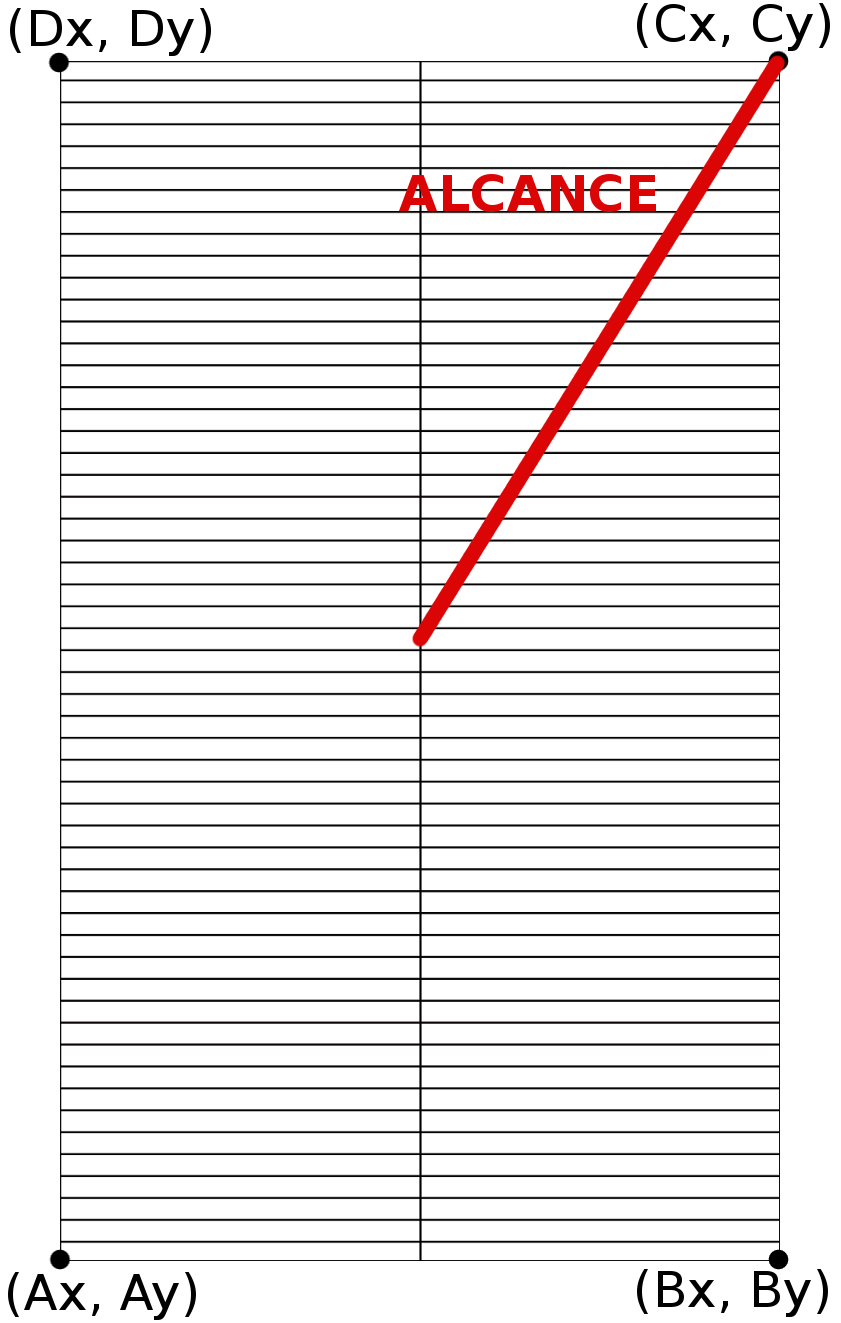
\includegraphics[width=0.5\linewidth]{CSU-vertices}
\caption{Vértices de la CSU}
\label{fig:vertices}
\end{figure}

%%%%%%%%%%%%%%%%%%%%%%%%%%%%%%%
\subsubsection{Métodos relevantes de \texttt{CSU}} \label{subsec:CSUmet}
Uno de los métodos más importantes de esta clase es aquél en el que se decide si
un objeto está dentro o no del apuntado. El método utiliza una simplificación 
del método conocido como ``ray casting'', utilizado en el desarrollo de
videojuegos para determinar colisiones entre polígonos. Este método verifica si
un punto se encuentra situado a la izquierda o a la derecha de uno de los
vértices del polígono. 
En nuestro caso, si un objeto se encuentra a la izquierda
de todas las aristas que forman el rectángulo del apuntado, significa que está
dentro del mismo. 
El código que comprueba esto es la función auxiliar
\texttt{estaDentro2}, que se muestra en el Listado \ref{codigo:csu0}.

\begin{lstlisting}[float=tp,language=C++, basicstyle=\ttfamily\footnotesize,caption={Código del ray casting simplificado},label={codigo:csu0}]                  
#define edge(x1, y1, x2, y2) (-(y2-y1) * p.getx() + (x2 - x1) * p.gety() - (-(y2-y1)*x1 + (x2-x1)*y1))
bool CSU::estaDentro2(const Element &p) const {
  set<Element>::iterator it = puntos.find(p);
  if (it != puntos.end())
    return false;
  register double distancia = (double)sqrt((p.getx() - x) * (p.getx() - x) + (p.gety() -y) * (p.gety() -y));
  if (distancia <= ALCANCE) {
    static int D1, D2, D3, D4;
    D1 = edge(Ax, Ay, Dx, Dy);
    D2 = edge(Dx, Dy, Cx, Cy);
    D3 = edge(Cx, Cy, Bx, By);
    D4 = edge(Bx, By, Ax, Ay);
    return (D1 <= 0 && D2 <= 0 && D3 <= 0 && D4 <= 0);
  }
  return false;
}

\end{lstlisting}

$ALCANCE$ es una constante cuyo valor corresponde a la distancia entre
el centro del apuntado y cualquiera de sus vértices (ver Figura
\ref{fig:vertices}. Si un punto está a una
distancia superior a esa, está fuera del radio de acción de la CSU, por lo que
no podrá estar dentro sea cual sea el ángulo $\alpha$ del apuntado. Si un objeto
se encuentra entre los vértices, se comprueba de que su posición sea válida
respecto a las barras. 
Esto se hace en la función pública \texttt{estaDentro},
cuyo código se muestra en el Listado \ref{codigo:csu1}.

\begin{lstlisting}[float=tp,language=C++,basicstyle=\ttfamily\footnotesize,
                   caption={Función que comprueba si un objeto está en la CSU},
                   label={codigo:csu1}]                  
int CSU::estaDentro(const Element &p, int &barra, double &distancia, double &rango) const {
  static double new_x, new_y, zone;
  if (estaDentro2(p)) {
    testeo(p, new_x, new_y);
    zone = sqrt((Ax - new_x) * (Ax - new_x) + (Ay - new_y) * (Ay - new_y));
	  barra = (int)(zone / DIST_BARRAS);
    if (barra == NUM_BARRAS)
      return 0;
    rango = zone - (barra * DIST_BARRAS);
    distancia = (double)sqrt((p.getx() - new_x) * (p.getx() - new_x) 
                           + (p.gety() - new_y) * (p.gety() - new_y));
    if (distancia > 2*ANCHO)
      return 0;
    if (barras_ocupadas[barra]) 
      return p_potencial(rango, barra);
    //Evitamos que esten justo donde van las barras
    static double redondeo; //demasiada precision en doubles
    redondeo = ceil(rango * PRECISION) / PRECISION;
    if (redondeo < BORDE_INF_DEF || redondeo > BORDE_SUP_DEF){
      return p_potencial(rango, barra);
    }
    //Miramos los bordes (1 arcseg por cada lado)
    if (conf.noborder) 
      if (redondeo <= BORDE_INF || redondeo >= BORDE_SUP)
        return p_potencial(rango, barra);
    if (conf.beamswitching) {
      if (orientacion == ARRIBA) 
        if (redondeo < BARRA2_3)
          return p_potencial(rango, barra);
      if (orientacion == ABAJO)
        if (redondeo > BARRA1_3)
          return p_potencial(rango, barra);
    }
    return !barras_ocupadas[barra];
  }
  return 0;
}
\end{lstlisting}

La función \texttt{testeo} calcula el punto de intersección entre la recta
formada por los vértices A y D de la CSU (lado izquierdo) y un objeto dado.
Cuando el método \texttt{estaDentro} comprueba que el punto coincide
perfectamente con una barra libre, devuelve el valor 1, en caso contrario hace
una llamada al método \texttt{p\_potencial}, que comprueba si el objeto podría
pertenecer al apuntado si se le realizara un mínimo movimiento de ajuste al
mismo. Dicho método devuelve los valores que aparecen en la Tabla
\ref{table:val_posibles}.

\begin{table*}[!ht]
\centering
\begin{tabular}{||l||c|c||}
\hline
\hline
 & Objeto en parte superior & Objeto en parte inferior \\
\hline
\hline
Barra actual libre &  2 & 5 \\
\hline
Barra superior libre & 3 & 0 \\
\hline
Barra inferior libre & 0 & 4 \\
\hline
\hline
\end{tabular}
\caption{Posibles valores del método \texttt{p\_potencial}}
\label{table:val_posibles}
\end{table*}

Los resultados pares indican que se ha de subir el centro del apuntado, de
manera que los objetos ``bajen'', los resultados impares implican lo contrario,
y el valor 0 indica que ese punto no puede pertenecer a la CSU puesto que no ha
superado las condiciones necesarias. Las restricciones que se usan se pueden observar
en el Listado \ref{codigo:csu2}.

\begin{lstlisting}[float=tpb,
                   language=C++,basicstyle=\ttfamily\footnotesize, 
                   caption={Función que comprueba si un objeto podría estár en la CSU},
                   label={codigo:csu2}]
int CSU::p_potencial(const double &rango, int &barra) const {
  if (rango > limiteS) { //Parte superior de la barra
    if (!barras_ocupadas[barra] && rango - limiteS + 0.01 <= margenDown)
      return 2;
    if (barra < NUM_BARRAS-1 && !barras_ocupadas[barra+1])
      if (DIST_BARRAS - rango + limiteI + 0.01 <= margenUp) {
        barra++;
        return 3;
      }
  }
  if (rango < limiteI) { //Parte inferior de la barra
    if (limiteI - rango + 0.01 <= margenUp) {
      if (barras_ocupadas[barra])
        return 0;
      else
        return 5;
    }
    if (barra > 0 && !barras_ocupadas[barra-1])
      if (rango + (DIST_BARRAS-limiteS) + 0.01 <= margenDown) {
        barra--;
        return 4;
      }
  }
  return 0;
}
\end{lstlisting}

Cuando un punto se ajusta perfectamente con una barra y no hay que mover el apuntado,
se utiliza el método \texttt{pointAdd}, que comprueba los límites y márgenes
del apuntado respecto al nuevo punto, lo introduce en el conjunto de puntos que
componen el apuntado y marca la barra en la que se encuentra como ocupada. Sin
embargo, cuando hay que hacer ajustes mínimos para que el objeto pueda ser
introducido, se utiliza la función \texttt{pointAddMove}, cuya implementación se
muestra en el Listado \ref{codigo:csu3}.

\begin{lstlisting}[float=tpb,
                   language=C++,basicstyle=\ttfamily\footnotesize,
                   caption={Método que añade un punto que requiere de ciertos ajustes},
                   label={codigo:csu3}]
void CSU::pointAddMove(Element &p, const int &move) {
  static double dist;
  if (move == 2 || move == 4) { //Hay que subir la CSU
    if (move == 2) //esta muy arriba
      dist = p.getzona() - limiteS + 0.01;
    if (move == 4)  //pasar a barra inferior
      dist = p.getzona() + (DIST_BARRAS - limiteS) + 0.01;
    if (alfa == CERO) { //es vertical, subimos la Y
      y += dist;
    }
    else if (alfa == PIMEDIO) { //es horizontal, movemos la X
      x -= dist;
    }
    else {
      static double raiz;
      raiz = sqrt((dist*dist)/(1 + ma * ma));
      y -= ma * raiz;
      x -= raiz;
    }
    margenDown -= dist;
    margenUp += dist;
  }
  else { //Hay que bajar la CSU
    if (move == 3)  //Pasar a barra superior 
      dist = DIST_BARRAS - p.getzona() + limiteI + 0.01;
    if (move == 5) { //Esta demasiado abajo
      dist = limiteI - p.getzona() + 0.01;
    }
    if (alfa == CERO) { //es vertical, bajamos la Y
      y -= dist;
    }
    else if (alfa == PIMEDIO) { //es horizontal, movemos la X
      x += dist;
    }
    else {
      static double raiz;
      raiz = sqrt((dist*dist)/(1 + ma * ma));
      y += ma * raiz;
      x += raiz;
    }
    margenDown += dist;
    margenUp -= dist;
  }
  extremos();
  puntos.insert(p);
  barras_ocupadas[p.getbarra()] = true;
  if (p.getprior() < prior)
    prior = p.getprior();
  actualizar2();
}
\end{lstlisting}

En la función \texttt{pointAddMove} se calcula cuál es la distancia mínima necesaria para que el
objeto pueda ser introducido, dependiendo de la opción en la que se encuentre el
mismo (véase la Tabla \ref{table:val_posibles}). Una vez movido el centro de la
\texttt{CSU} se invocan dos métodos muy importantes de esta clase. El primero,
\texttt{extremos}, recalcula la posición de los vértices del apuntado, puesto
que se ha movido de sitio; y el segundo, \texttt{actualizar2}, se encarga de
comprobar de nuevo todos aquellos atributos que dependen de la posición de los
objetos, tales como las distancias mínimas recogidas en el atributo
\texttt{distancia\_punto} o los nuevos márgenes de movimiento del apuntado.

En el Capítulo \ref{chap:algorithm} se hacía referencia a una serie de movimientos de mejora
que se podían efectura sobre la \texttt{CSU}, con el objetivo de abarcar un mayor número de objetos.
Estos posibles movimientos son cuatro y se agrupan en dos: movimientos
verticales y movimientos horizontales. En los primeros, se produce un cambio de
barra de los objetos, situando aquél que se encuentre en la barra más cercana al
borde inferior de la \texttt{CSU} en la barra 0 del apuntado (en el caso de la mejora
hacia arriba) o trasladando el objeto que ocupa la barra más cercana al borde
superior en la última barra (en el otro caso). En este tipo de movimiento la
zona de la barra en la que se encuentra un objeto no se ve afectada. Por el
contrario, en el segundo tipo de movimiento, el horizontal, lo que no se ve
afectado es la barra de cada uno. En este caso lo que se persigue es mover los
objetos hasta el borde izquierdo o derecho del apuntado, obteniendo una nueva
área de búsqueda alrededor de la \texttt{CSU}. Nuevamente se ha de llamar al método
\texttt{extremos} para calcular los nuevos vértices del apuntado con cada
movimiento. En el Listado \ref{codigo:csu4} se muestra un ejemplo de cada uno de
los tipos de mejora mencionados.

\begin{lstlisting}[float=tpb,
                   language=C++, basicstyle=\ttfamily\footnotesize, 
                   caption={Código del movimiento de mejora vertical hacia arriba},
                   label={codigo:csu4}]
void CSU::mejoraArriba() {
  static int i, j, z;
  static double dist;
  i = CERO;
  while (!barras_ocupadas[i])
    i++;
  if (i != CERO) {
    for (j = CERO; j+i < NUM_BARRAS; j++){
      barras_ocupadas[j] = barras_ocupadas[j+i];
    }
    for (j = NUM_BARRAS - i; j < NUM_BARRAS; j++){
      barras_ocupadas[j] = false;
    }
    dist = i * DIST_BARRAS;
    if (alfa == CERO) { //es vertical, subimos la Y
      y += dist;
    }
    else if (alfa == PIMEDIO) { //es horizontal, movemos la X
      x -= dist;
    }
    else {
      static double raiz;
      raiz = sqrt((dist*dist)/(1 + ma * ma));
      y -= ma * raiz;
      x -= raiz;
    }
    extremos();
    actualizar(-i);
  }
}
\end{lstlisting}

\begin{lstlisting}[float=tpb,
                   language=C++, basicstyle=\ttfamily\footnotesize,
                   caption={Código del movimiento de mejora horizontal izquierdo},
                   label={codigo:csu5}]
void CSU::mejoraIzquierda() {
  static int j;
  static double dist;
  if (dist_min > 0.2) {
  dist = dist_min - 0.1;
  if (alfa == CERO) { //es vertical, movemos la X
    x += dist;
  }
  else if (alfa == PIMEDIO) { //es horizontal, movemos la Y
    y += dist;
  }
  else {
    static double raiz;
    raiz = sqrt((dist*dist)/(1 + mb * mb));
    if (alfa < PIMEDIO) {
      x += raiz;
      y += mb * raiz;
    } else {
      x -= raiz;
      y -= mb * raiz;
    }
  }
  extremos();
  actualizar(0);
  }
}
\end{lstlisting}

En ambos casos se utiliza la función \texttt{actualizar}, que funciona de modo
análogo a \texttt{actualizar2}, actualizando los objetos y el contenido de los
atributos.

El método \texttt{colision} es otra de las claves de esta clase, pues se encarga
de determinar si entre dos apuntados existe una colisión o solape. La forma de
comprobarlo es mediante proyecciones de planos e intersecciones de rectas: se
proyectan los vértices de una \texttt{CSU} $B$ sobre las rectas definidas por
los vértices AD y AB de la \texttt{CSU} $A$. Si en alguna de estas proyecciones
el rango dado por el par de vértices (mínimo y máximo) proyectados no tiene
puntos en común con el rango formado por el par de vértices AD, o AB según el
caso, podemos afirmar que no hay colisión. En caso de no poder realizar tal
afirmación, comprobamos si existe algún punto de $A$ en $B$, en cuyo caso se
afirmaría que existe un solapamiento entre ambas. Se debe tener en cuenta que
aunque se llegue al final del método y no haya ningún punto de $A$ en $B$, es
posible que sí haya alguno de $B$ en $A$, por lo que se debe hacer doble
comprobación. El código de este método se muestra en el Listado
\ref{codigo:csu6}.

\begin{lstlisting}[float=tpb,
                   language=C++, basicstyle=\ttfamily\footnotesize, numbers=none,
                   caption={Código del método que comprueba las colisiones},
                   label={codigo:csu6}]
bool CSU::colision (const CSU &csu) const {
  csu.getABCD(s2);  //Ax,Ay,Bx,By,Cx,Cy,Dx,Dy
  //RECTA AD
  for (i = 0; i < 8; i+=2) { //cada uno de los puntos de CSU2
    if (alfa != CERO && alfa != PIMEDIO) { // No es ni vertical ni horizontal
      punto.first = (ma * Ax - mb * s2[i] + s2[i+1] - Ay) / (ma - mb);
      punto.second = ma * (punto.first - Ax) + Ay;
    }
    else if (alfa == CERO){   // Es vertical
      punto.first = Ax;
      punto.second = s2[i+1];
    }
    else{  // Es horizontal
      punto.first = s2[i];
      punto.second = Ay;
    }
    minimoX = min(minimoX, punto.first);
    maximoX = max(maximoX, punto.first);
    minimoY = min(minimoY, punto.second);
    maximoY = max(maximoY, punto.second);
  }
  //Comprobamos que no haya solape
  miX = min(Ax,Dx); maX = max(Ax,Dx);
  if (maximoX < miX)
    return false;
  if (minimoX > maX)
    return false;
  miX = min(Ay,Dy); maX = max(Ay,Dy);
  if (maximoY < miX)
    return false;
  if (minimoY > maX)
    return false;
  //Repetimos para el lado DC
  //Comprobamos si los puntos colisionan
  CSU vacia (csu.getx(), csu.gety(), csu.getalfa());
  for (p = puntos.begin(); p != puntos.end(); p++)
    if (vacia.estaDentro(*p,b,d,z))
      return true;
  return false;
}
\end{lstlisting}
%%%%%%%%%%%%%%%%%%%%%%%%%%%%%%%
\subsection{La clase \texttt{Parser}}
\texttt{Parser} hereda de la clase \texttt{SaxParser}, definida en la librería
\texttt{libxml++}, cuya función es actuar como un parser de XML. 
\texttt{Parser} es una adaptación a nuestro problema particular de los métodos que aparecen en la
documentación de la librería. Sus objetivos son los de comprobar que la
estructura del fichero de entrada a \CSUO{} sea el correcto y devolver los
datos contenidos en dicha entrada en las estructuras explicadas anteriormente.
La estructura del fichero de entrada es la que se muestra en el Listado
\ref{codigo:xml-in}.

\begin{lstlisting}[float=tpb,
                   numbers=none,
                   language=XML,
                   caption={Estructura de los ficheros de entrada para \CSUO{}},
                   label={codigo:xml-in}]
<Observables [widht=``Ancho_cielo'' height=``Alto_cielo'']>
    <Element id=``Identificador''>
        <X>PosX</X>
        <Y>PosY</Y>
        <Prioridad>[1..99]</Prioridad>
    </Element>
<!-- ...  -->
</Observables>
\end{lstlisting}

En el Listado \ref{codigo:xml-exacto} se muestra un extracto de un ejemplo de entrada con datos
reales, extraídos del fichero \texttt{exacto.xml}.

\begin{lstlisting}[float=tpb,
                   numbers=none,
                   language=XML,
                   caption={Ejemplo de entrada para \CSUO{},
                   extraído de \texttt{exacto.xml}},
                   label={codigo:xml-exacto}]
<Observables widht="900" height="900">
	<Element id="0">
		<x>573</x>
		<y>402.4242</y>
		<Prioridad>1</Prioridad>
	</Element>
	<Element id="1">
		<x>595</x>
		<y>409.6968</y>
		<Prioridad>1</Prioridad>
	</Element>
	<Element id="2">
		<x>458</x>
		<y>416.9694</y>
		<Prioridad>1</Prioridad>
	</Element>
	<Element id="3">
		<x>409</x>
		<y>424.242</y>
		<Prioridad>1</Prioridad>
	</Element>
<!-- ...  -->
	<Element id="54">
		<x>409</x>
		<y>795.1446</y>
		<Prioridad>1</Prioridad>
	</Element>
</Observables>
\end{lstlisting}

Los datos facilitados a la aplicación han de estar en arcosegundos, y nunca con
valores negativos. 
En caso de tener una instancia de entrada que no cumpla este requisito puede
utilizarse el conversor que se explica en la Sección \ref{sec:conver}.

%%%%%%%%%%%%%%%%%%%%%%%%%%%%%%%
\subsubsection{Atributos de \texttt{Parser}}
\begin{itemize}
\item \texttt{Q}: conjunto de objetos contenidos en el fichero de entrada.
\item \texttt{fich}: fichero XML de entrada.
\item \texttt{punto}: objeto donde se crean las instancias de los elementos
contenidos en el archivo entrante.
\item \texttt{nodo}: identificador del  nodo en el que se encuentra el
analizador durante el procesado.
\item \texttt{nuevo}: indica el nivel de procesado que lleva en la estructura,
en nuestro caso cuando llega a 3 se determina que ha completado un elemento.
\item \texttt{widht, height}: ancho y alto especificados para definir el tamaño
de la pantalla de Allegro.
\end{itemize}
%%%%%%%%%%%%%%%%%%%%%%%%%%%%%%%
\subsubsection{Métodos relevantes de \texttt{Parser}}
Cuando se construye una instancia de esta clase comienza el procesado del
archivo especificado por parámetro. En el constructor se comprueba línea a línea
si el fichero sigue la estructura especificada, mediante llamadas a las funciones
virtuales de la clase. Éstas son métodos que especifican qué se comprueba en
cada nivel y cuando se ha terminado de construir un objeto para añadirlo a
\texttt{Q}. El método que realmente interesa es \texttt{getList}, que
devuelve el conjunto de datos de entrada del problema.

%%%%%%%%%%%%%%%%%%%%%%%%%%%%%%%
\subsection{La clase \texttt{Dbscan}} \label{sec:dbscan}
Esta es la clase que implementa el algoritmo descrito en la Sección
\ref{sec:clustering}. El código de \texttt{Dbscan} es el resultado de una
adaptación y traducción a C++ de un código Java que implementaba este algoritmo de clustering.
Se ha mantenido el tipo de los atributos para evitar alterar el correcto
funcionamiento del código. 

Los objetos (de la clase \texttt{Element}) se agrupan en vectores, definidos en
la clase estándar \texttt{vector} de C++. 
Este contenedor agrupa los objetos por orden de llegada. 

%%%%%%%%%%%%%%%%%%%%%%%%%%%%%%%
\subsubsection{Atributos de \texttt{Dbscan}}
\begin{itemize}
\item \texttt{e}: indica la distancia utilizada en el cálculo de vecindades.
\item \texttt{minpt}: mínimo de puntos que forman un núcleo.
\item \texttt{resultList}: vector de listas de vectores de elementos. Cada lista
representa un clúster de puntos.
\item \texttt{pointList}: es el conjunto de datos de entrada.
\end{itemize}
%%%%%%%%%%%%%%%%%%%%%%%%%%%%%%%
\subsubsection{Métodos relevantes de \texttt{Dbscan}}
Se utiliza \texttt{setList} y \texttt{getList} para establecer u obtener el
conjunto de objetos de entrada, y el método \texttt{start} para comenzar el
proceso de agrupamiento de los objetos. Para obtener el vector de resultados,
contenido en el atributo \texttt{resultList} se usa el método
\texttt{getResult}.
%%%%%%%%%%%%%%%%%%%%%%%%%%%%%%%
\subsection{Algoritmos principales}

El archivo \texttt{main.C} organiza el uso de todas las clases descritas para
implementar el algoritmo constructivo planteado en la Sección
\ref{sec:algconst}. El código para crear la solución inicial de dicho algoritmo
es el que se presenta en el Listado \ref{codigo:main1}.

\begin{lstlisting}[float=tpb,
                   language=C++, numbers=none,
                   caption={Primera fase del algoritmo constructivo: generar la solución inicial},
                   label={codigo:main1}]
set<CSU> diferentes[5];
sort(diferentes[0],TAMPUN);
int mej, min = MAX;
CLOCK_Start(chrono);
for (int i = MENORX; i < 5; i++) {
  diferentes[i] = apuntadosRandom(parser.getList(), i);
  if (diferentes[i].size() < min) {
    min = diferentes[i].size();
    mej = i;
  }
}
set<CSU> centros = diferentes[mej];
\end{lstlisting}

En el Listado \ref{codigo:main2} se detalla la función \texttt{apuntadosRandom},
encargada de generar varias soluciones del problema sobre las que se elige la
mejor.

\begin{lstlisting}[float=tpb,
                   language=C++, numbers=none,basicstyle=\ttfamily\footnotesize,
                   caption={Código de la función que genera soluciones
                   aleatorias},
                   label={codigo:main2}]
set<CSU> apuntadosRandom(set<Element> puntos, const int &opcion) {
  static set<Element>::iterator v;
  static set<CSU> posibles;
  set<CSU> resultado;
  posibles.clear();
  static set<CSU>::iterator i;
  static CSU mejor_opcion;
  static int contador;
  if (opcion <= 4) {
    sort(puntos, opcion);
    set<Element> eliminados;
    set<Element> cluster = puntos;
    static set<Element>::iterator e1;
    while (!puntos.empty()) 
      for (v = cluster.begin(); v != cluster.end(); v++) { 
        progreso();
        e1 = eliminados.find(*v);
        if (e1 == eliminados.end()) {
          posibles = selectAP(*v, puntos);
          i = posibles.begin(); 
          mejor_opcion = *i; 
          resultado.insert(mejor_opcion);
          eliminar_puntos(mejor_opcion.getPoints(), puntos, eliminados); 
        }
      }
  }
	// ... //
  return resultado;
}
\end{lstlisting}

La segunda fase, en la que se realiza el proceso de eliminar solapes entre
apuntados, se realiza dentro de \texttt{colisiones}. Este método se encuentra
detallado en el Apéndice \ref{app:colis} debido a su extensión.

La implementación del algoritmo \texttt{GRASP} definido en la Sección
\ref{sec:grasp} se encuentra en la función \texttt{grasp} del fichero
\texttt{main.C}, mostrada en el Apéndice \ref{app:grasp}.

%%%%%%%%%%%%%%%%%%%%%%%%%%%%%%%
\section{Modo de empleo de \CSUO{}} \label{sec:uso_app}

Para utilizar \CSUO{} una vez compilada (usando \texttt{make}),
hay que especificar una serie de opciones y un archivo \texttt{XML} con los
objetos de entrada.

\begin{lstlisting}[numbers=none]
$ ./csuoptimizer [opciones] entrada.xml
\end{lstlisting}

Las opciones disponibles en \CSUO{} son: 
\begin{itemize}
\item \texttt{--help}: Muestra una ayuda con las opciones disponibles y un
ejemplo de uso.
\item \texttt{--dbscan}: indica a \CSUO{} que se quiere hacer uso
del algotimo DBScan explicado en la Sección \ref{sec:dbscan}. Desactivado por
defecto.
\item \texttt{--grasp}: habilita el uso de la heurística GRASP para intentar
mejorar la solución. Desactivada por defecto.
\item \texttt{--graphic}: muestra en la ventana generada por Allegro los pasos
que está realizando \CSUO{} durante su ejecución. Este paso está
pensado para labores de depuración y desarrollo y ralentiza la ejecución de la
aplicación.
\item \texttt{-NR}: especifica el número de rotaciones que hará una CSU durante
el proceso de búsqueda de objetos inicial. Por defecto este valor es igual a 20,
pues se han obtenido buenos resultados en todos los ejemplos. Un ejemplo de su
uso sería \texttt{./csuoptimizer -NR 15 entrada.xml}.
\item \texttt{--verbose}: genera un archivo \texttt{verbose.txt} con información
de control, útil para depuración y desarrollo.
\item \texttt{--dat}: indica el modo de salida de los resultados. Por defecto se
usa el formato \texttt{XML}, cuyo ejemplo se puede ver en el Anexo
\ref{app:exacto.xml}, sin embargo es posible que el usuario requiera de otro
tipo de salida. Esta estructura adicional se muestra en el Listado
\ref{codigo:exacto.dat}.
\item \texttt{--beams}: habilita el uso del \texttt{beam switching}.
\item \texttt{--noborder}: especifica que no se quieren objetos cercanos a la
barra, por lo que se deshabilita un espacio de 1 arcosegundo en cada uno de los
bordes.
\end{itemize}


\begin{lstlisting}[float=tpb,
                   numbers=none,mathescape,
                   caption={Estructura del modo de resultado \texttt{.dat}},
                   label={codigo:exacto.dat}]
**************************************************************
coordenadaX			coordenadaY			anguloInclinacion
				posicionBarra_1
				posicionBarra_2

				   $\vdots$

				posicionBarra_55
**************************************************************
coordenadaX			coordenadaY			anguloInclinacion

    $\vdots$

\end{lstlisting}

Las opciones \texttt{--beams} y \texttt{--noborder} afectan al área útil de una
barra. En la Figura \ref{fig:barras} se muestran los casos posibles de una
barra. La zona blanca es la zona útil de barra, donde se puede detectar un
objeto, la zona en color gris hace referencia al área eliminada por el usuario
mediante las opciones.

\begin{figure}[!htb]
\centering
\subfloat{

\includegraphics[width=0.2\linewidth]{BarraPunto1}}
\subfloat{

\includegraphics[width=0.2\linewidth]{BarraPunto2}}
\subfloat{

\includegraphics[width=0.2\linewidth]{BarraPunto3}}
\subfloat{

\includegraphics[width=0.2\linewidth]{BarraPunto4}}
\caption{Disponibilidad de las barras según las opciones de entrada. a) Barra
normal. b) Barra con \texttt{--noborder}. c) Barra con \texttt{--beams}. d)
Barra con ambas opciones}
\label{fig:barras}
\end{figure}

%%%%%%%%%%%%%%%%%%%%%%%%%%%%%%%
\section{Herramientas de apoyo}
Con el objetivo de comprobar el buen funcionamiento de \CSUO{} y
de facilitar al usuario herramientas útiles que permitan una mayor
familiarización con la aplicación, se aportan dos herramientas complementarias
explicadas en las siguientes Secciones.
%%%%%%%%%%%%%%%%%%%%%%%%%%%%%%%
\subsection{``Editor de mapas''}
En el directorio \texttt{map\_editor} del proyecto se encuentra un programa \texttt{mapEditor} que
genera entradas para el \CSUO{} con apuntados específicos. 
Los ejemplos sintéticos que se presentan en la Sección \ref{sec:sintetico} de esta
Memoria han sido generados mediante esta aplicación. Se cuenta con un archivo
\texttt{Makefile} para automatizar la compilación.

El \texttt{mapEditor} generado por la compilación muestra un menú por consola
con las siguientes opciones:
\begin{itemize}
\item \texttt{1 Crear CSU}: permite especificar la posición de una CSU así como
su ángulo de inclinación. Automáticamente se añade un objeto en cada barra de
forma aleatoria. La pantalla gráfica de esta aplicación tiene un tamaño de
$900\times900$ arcosegundos, por lo que se deben introducir valores en este
rango para poder visualizarlos.
\item \texttt{2 Visualizar CSUs}: muestra la disposición de las CSUs en el
espacio visible.
\item \texttt{3 Visualizar Puntos}: muestra únicamente la nube de objetos
generada, la cual será la entrada a la aplicación \CSUO{}.
\item \texttt{4 Visualizar Espacio}: muestra de manera conjunta las dos opciones
anteriores, es decir, cada apuntado con sus respectivos objetos.
\item \texttt{5 Guardar puntos}: genera un archivo \texttt{XML} con los objetos
creados, el cual será el fichero de entrada de \CSUO{}.
\item \texttt{6 Salvar datos}: guarda el estado actual de la aplicación en un
fichero \texttt{save.dat} para reutilizarlo cuando convenga.
\item \texttt{7 Cargar datos}: carga en memoria un estado antiguo de la
aplicación desde un fichero especificado por el usuario.
\end{itemize}
%%%%%%%%%%%%%%%%%%%%%%%%%%%%%%%
\subsection{Conversor} \label{sec:conver}
Los ejemplos facilitados por el responsable del proyecto EMIR no se presentan en
el formato de entrada requerido por \CSUO{}, razón por la que se ha
incluido un conversor que:
\begin{itemize}
\item transforma un fichero con datos en texto plano agrupados por columnas (véase
el Listado \ref{codigo:estructdat}) al formato de entrada requerido.
\item realiza un cambio de coordenadas para evitar valores negativos en
\CSUO{}.
\item permite cambiar de grados a arcosegundos con la opción \texttt{-g2a}.
\end{itemize}

Esta herramienta genera dos archivos de salida:
\begin{itemize}
\item Uno con la misma estructura que la entrada, es decir, la que se muestra en
el Listado \ref{codigo:estructdat}, terminado en \texttt{-converted.dat} en
\texttt{ejemplos/} para que se tenga un control de cambios en los objetos debido
al cambio del centro de origen.
\item Un fichero con el mismo nombre que el de origen pero en XML situado en
\texttt{ejemplos/xml/} listo para su uso en \CSUO{}.
\end{itemize}

Ejemplo de uso:
\begin{lstlisting}[float=tpb,
                   numbers=none]
./conversor-dat-xml [-g2a] archivo.dat
\end{lstlisting}

\begin{lstlisting}[caption={Estructura de entrada de los ficheros .dat},
                  label={codigo:estructdat}]
posicionXobjeto1  posicionYobjeto1  prioridadObjeto1
posicionXobjeto2  posicionYobjeto2  prioridadObjeto2

      ...               ...               ....

posicionXobjetoN  posicionYobjetoN  prioridadObjetoN
\end{lstlisting}
